\chapter{Results}

In this chapter we will show the results obtained from the solution of two design optimization problems related to:
\begin{itemize}
	\item a simple $1$D segment;
	\item the shape of a face of a cube.
\end{itemize}
These has been formulated as optimization problems and the adjoint method was used to compute the gradient of the corresponding cost functions throughout the optimization.

However, since both optimization problems are built on top of physical systems described by means of Poisson equations, we will first briefly describe this equation in a dedicated section before delving deeper into them.

\section{Poisson Equation}
\label{sec:poisson_equation}

Given a region $\Omega \subset \R^d$, with $d \in \N$ and bounded by the boundary $\partial\Omega$, the generic heat equation with internal heat generation~\cite{Brezis:functional_analysis_book}, at steady state, is described by the Poisson Equation which is defined by the following Partial Differential Equation (PDE):
\begin{equation}
	\label{eqn:Poisson_equation}
	\begin{cases}
		- \Delta u(\vec{x}) = f(\vec{x})														 &  \text{in $\Omega$}							\\
		\mathcal{B} u(\vec{x}) = g(\vec{x})  													 &  \text{on $\partial\Omega$}
	\end{cases}
\end{equation}
where $\Delta$ indicates the Laplacian operator, $\mathcal{B}$ is the (possibly differential) generic linear operator that enforce the boundary conditions (BCs) and $f$ and $g$ are known functions.
The Poisson equation is a well-known example of a PDE that can be effectively addressed using meshless techniques, such as the RBF-FD approach detailed in this work.

We decided to evaluate the results of the adjoint method applied to RBF-FD method on the aforementioned equation due to both its wide range of applications in different areas	(e.g. electrostatic, chemistry, gravitation and others) and the simplicity of its analytical manipulation.

%\medskip
%In particular for this thesis and to obtain the results presented in this chapter we implemented RBF-FD method as follow:
%\begin{itemize}
%%TODO: 	\item consider domains $\Omega \subset \R^{d}$ with $d=1,3$;  Da spostare nell'intro ai results
%	\item use RBFs augmented with polynomial terms as basis functions $B_k$ to approximate the solution $u$ in a similar way to what has been done in~\cite{Liu:Intro_to_meshfree_methods}; 
%	\item formulate the problem in its strong form, so we will use the collocation technique in combination with the Weighted Residual Method.
%\end{itemize}
%thus we will apply the RBF-generated Finite Differences (RBF-FD)~\cite{Fornberg:RBF-FD_1, Fornberg:RBF-FD_2} to solve~\eqref{eqn:Poisson_equation} in one and three dimensional physics domain.
% "Collocation methods with Weighted Residual Methods" Cioè prima hai citato i collocation, ma i weighted residual da dove saltano fuori?? Da spiegare meglio/togliere??
%
%Mono dimensional physics domain are used to gain confidence with the techniques explained while three dimensional  domain are used for their application in real case problems as those faced at Esteco. $2$D cases, instead, have been skipped in the analysis since they would only be used to bridge the 2 previous scenarios and therefore would have had no practical utility.
%
%RBFs are used for scattered data interpolation both for their physical foundation[overview 20, Hardy 1990] and for their profitable use in applications like meteorology, turbulence analysis and neural network~\cite{Chen:meshless_overview_after_20_years}
%
%Finally, collocation technique is employed because thanks to its ability to discretize the Boundary Value problem~\eqref{eqn:Poisson_equation} expressed in strong form leads to a real fully meshless approach~\cite{Miotti:RBF_in_depth}.


\section{1D case}

In this case $d=1$. The physical domain is simply a segment and its boundary consists on its two endpoints that we indicate with $a$ and $b$, both belonging to $\R$. Therefore we have $\Omega =~]a,b[$ and $\partial\Omega = \Set{a, b}$.
For the remaining portion of the boundary value problem we define $f(x) = - \omega^2 \sin(x)$ and we impose the following homogeneous BCs: $u(a)=0$ and $u(b)=0$. Fixing the values $\omega=1$, $a=0$ and $b=\pi$ allows to rewrite the Poisson equation reported in~\eqref{eqn:Poisson_equation} as
\begin{equation}
	\label{eqn:Poisson_equation_1D}
	\begin{cases}
		- \Delta u(\vec{x}) = - \sin(x) & \text{in $]a,b[$}  \\
		u(a) = 0  \\
		u(b) = 0
	\end{cases}
\end{equation}
In order to find an approximated solution to the problem~\eqref{eqn:Poisson_equation_1D} we employ the RBF-FD method parametrized as follow:
\begin{itemize}
	\item $N=41$ evenly spaced nodes are used for domain discretization: $N_I=39$ are placed in $\Omega$ and the other $N_B=2$ are placed repsectivelly in $a$ and $b$;
	\item $\varphi(r) = r^3$ Polyharmonic function is used as basic function to define the RBF interpolant;
	\item $P=2$ is the degree of its polynomial augmentation;
	\item $m=7$ is the number of nodes which constitute a single stencil;
\end{itemize}
As done previously we indicate with $\vec{u}_I$ the vector obtained by solving the system~\eqref{eqn:compact_discretized_PDE} derived from RBF-FD discretization.
%TODO: Sposta il vincolo dopo la cost function
The discretized version of equation~\eqref{eqn:Poisson_equation_1D} will be the constraints during the optimization

\smallskip
The design optimization problem, related to segment $[a,b]$, that we want to solve is the minimization of the following cost function:
\begin{equation}
	J(\vec{u}_I, b) = \frac{1}{2} \frac{b}{N-1} \left( \sum_{i=2}^{40} u(x_i) - E \right)^2
\end{equation}
where $E\in\R$ is a parameter set by us to a value of $2.5$ and $l=b$ is the single design variable. This particular configuration of the design variable means that in order to meet the objective we are allowed to vary the length of the segment $[a,b]$.
%$\vec{u}_I$ is the result of the simulation performed through the RBF-FD solver and
%We remind that the discretized version of Equation~\eqref{eqn:Poisson_equation_1D} will be a constraint during the optimization.

\smallskip
The results after $30$ steps in the optimization procedure are shown in figure~\ref{fig:opt_results_1D},

\begin{figure}
	\centering
	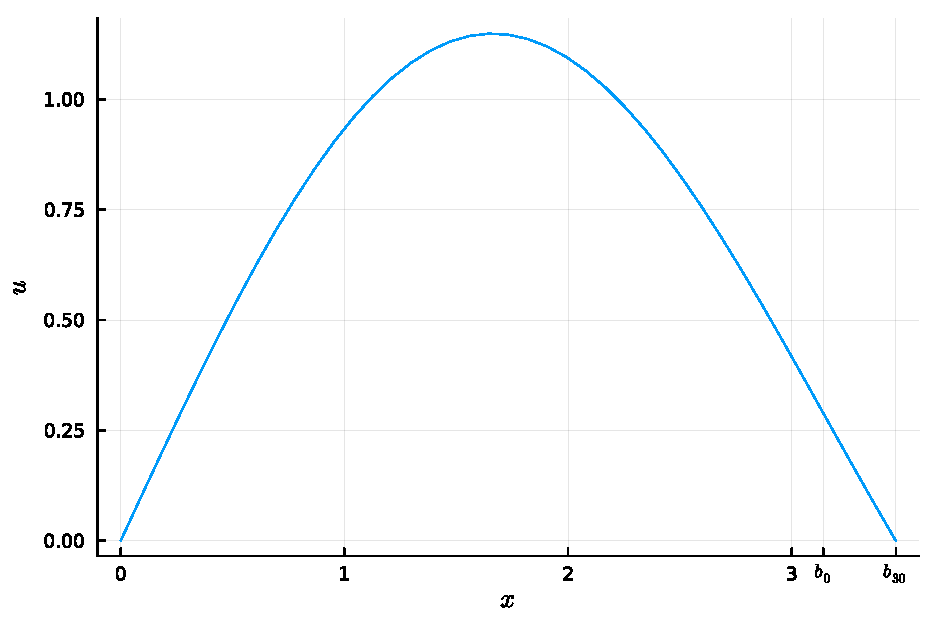
\includegraphics[width=.75\textwidth]{img/uOpt_vs_x_1D.pdf}
	\caption{discretized approximated solution obtained solving~\eqref{eqn:Poisson_equation_1D} via RBF-FD at the end of the design optimization. $b_0$ and $b_{30}$ indicate respectively the intial and the final position of the $b$ endpoint}
	\label{fig:opt_results_1D}
\end{figure}

\begin{figure}
	\centering
	\subfloat[][\emph{Cost function values}]
	{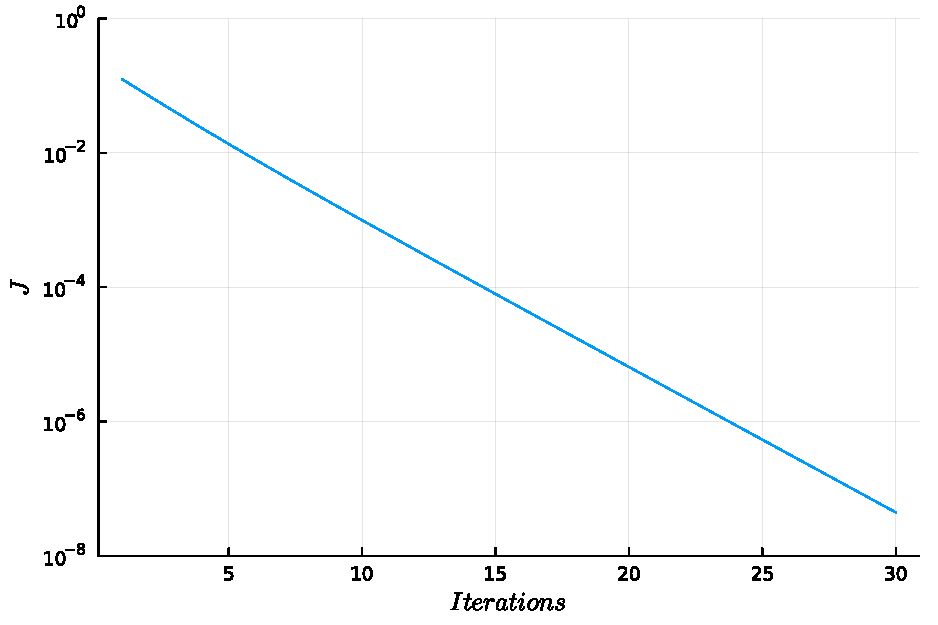
\includegraphics[width=.45\textwidth]{img/cost_vs_iter_1D.pdf}} \quad
	\subfloat[][\emph{Cost function gradient values}]
	{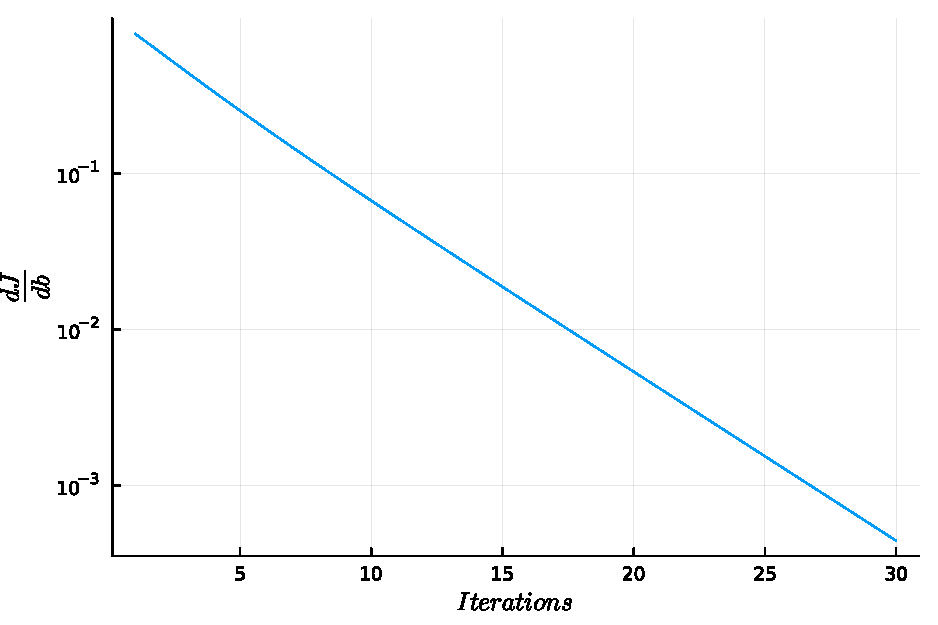
\includegraphics[width=.45\textwidth]{img/costGrad_vs_iter_1D.pdf}}
	\caption{Trajectories of the cost function and its gradient throughout the optimization process. The ordinates are on a logarithmic scale}
	\label{fig:opt_history_1D}
\end{figure}

while in figure~\ref{fig:opt_history_1D} are shown the dynamic of the cost function and of its gradient respect the design variable $b$.

%\begin{figure}
%	\centering
%	\subfloat[][\emph{Cost function values}]
%		{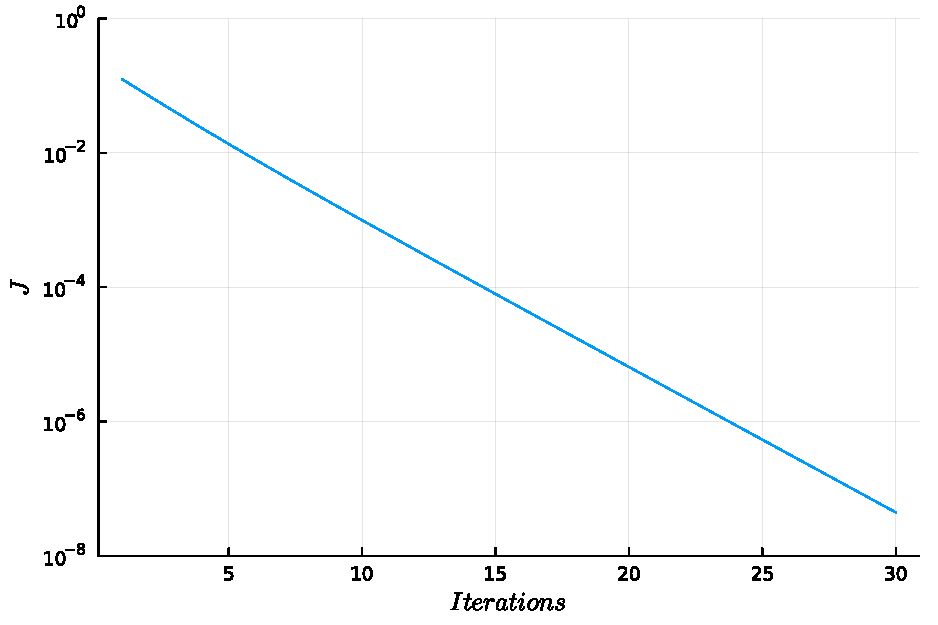
\includegraphics[width=.45\textwidth]{img/cost_vs_iter_1D.pdf}} \quad
%	\subfloat[][\emph{Cost function gradient values}]
%		{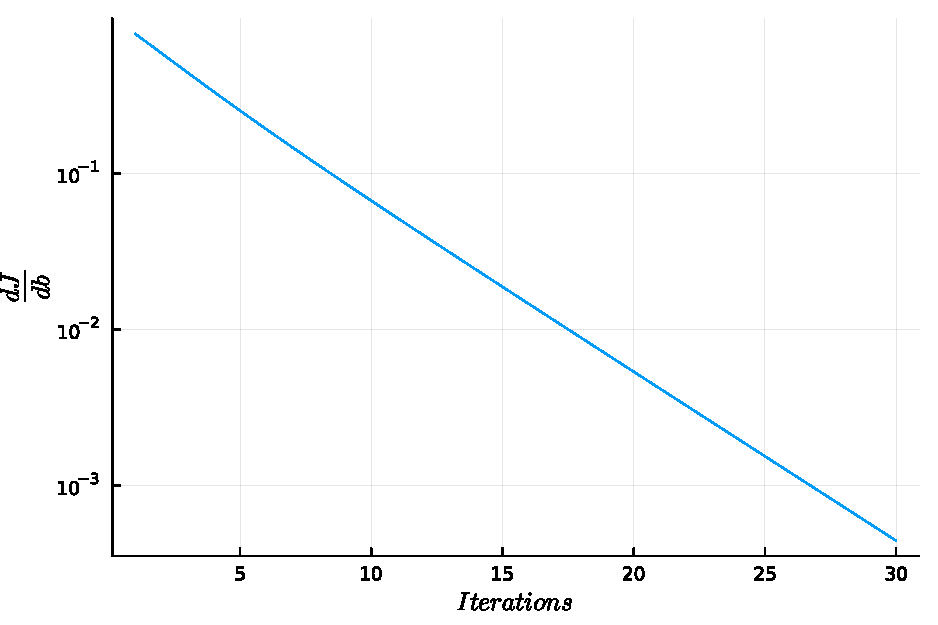
\includegraphics[width=.45\textwidth]{img/costGrad_vs_iter_1D.pdf}}
%	\caption{Trajectories of the cost function and its gradient throughout the optimization process. The ordinates are on a logarithmic scale}
%	\label{fig:opt_history_1D}
%\end{figure}



\section{3D case}
\label{sec:results_3D_case}

Now the physical domain $\Omega$ consists of a square-based prism with a side length of $1$ and a height of $0.5$, its faces are indicated with $\partial\Omega$. In particular $\partial\Omega$ is further partitioned in two subsets:
\begin{itemize}
	\item $\partial\Omega_\textup{flux}$ which is formed by the north face of the prism;
	\item $\partial\Omega_\textup{walls}$ which includes the remaining faces.
\end{itemize}
Figure~\ref{fig:3D_prism-shaped_domain} show a representation of the domain.

\begin{figure}[htp]
	\centering
	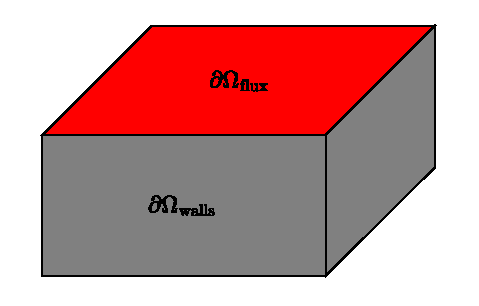
\includegraphics[width=.5\textwidth]{img/3D_prism-shaped_domain}
	\caption{Physical domain used for the $3$D Poisson equation. Boundaries $\partial\Omega_\textup{flux}$ and $\partial\Omega_\textup{walls}$ are highlighted in red and gray respectively}
	\label{fig:3D_prism-shaped_domain}
\end{figure}

The Poisson equation associated to the geometry is defined as:
\begin{equation}
	\label{eqn:3D_BV_problem}
	\begin{cases}
		\Delta u = - \omega^2 f  &  \text{in $\Omega$}  \\
		\frac{\partial u}{\partial \vec{n}} = \frac{\partial u}{\partial \vec{n}}  &  \text{in $\partial\Omega_\textup{walls}$}  \\
		u = f  &  \text{in $\partial\Omega_\textup{flux}$}  \\
	\end{cases}
\end{equation}
where $\vec{n}$ is the surface normal at the boundary and $f$ is defined as $f(\vec{x}) = \sin(\omega x)\sin(\omega y)\sin(\omega z)$, with $\vec{x} \in \Omega\cup\partial\Omega$ being a point in space with coordinates $x$, $y$ and $z$, and $\omega = 2\pi$. 

The problem under consideration allows for various physical interpretations: if we consider $u$ as the temperature and $-\omega^2 f$ as a generic heat source, the aforementioned problem constrains the temperature of the north face to be constant and to follow a profile defined by $f$ (Dirichlet BC), and impose a prescribed heath flux on the other faces (Neumann BC); by solving it we obtain the temperature values within the domain.

On top of the boundary value problem~\eqref{eqn:3D_BV_problem} a design optimization problem is subsequently formulated: we want to maximize the flux through the north wall per unit area by modifying the shape of the wall itself. This is the problem that we are going to solve in this section. The associated cost function can be defined in a similar way as was done in subsection~\vref{subsec:adjoint_method_RBF-FD_3D}:
\begin{equation}
	\label{eqn:continuous_3D_cost_function_results}
	J_c = \frac{1}{\abs{\partial\Omega_\text{flux}}} \int_{\partial\Omega_\textup{flux}} \frac{\partial u}{\partial \vec{n}} \, ds
\end{equation}
where $\abs{\partial\Omega_\text{flux}} \in \R$ is the area of the surface defined by $\partial\Omega_\text{flux}$.

%TODO: Da valutare il senso di questa frase. Infatti in questo caso è meglio toglierla che metterla.
%If we define the design variables as the height of each single point in $\partial\Omega_\text{flux}$ then we obtain an infinite-dimensional optimization problem which is infeasible to solve in practice.

In this case too a physical interpretation of the problem is possible: if we suppose we are dealing with a heat conduction problem, like in the example given earlier in this section, than the problem~\eqref{eqn:3D_design_opt_problem} is asking to find the best shape for the north face in order to maximize the average heat flux density with the exterior of the prism.

\medskip
However, in our case the geometry is not described by means of continuous quantities and it is separately defined in a \verb|.stl| file which characterize the surface of the prism using a triangular mesh as it is shown in figure~\ref{fig:3D_cube_stl_initial}.

\begin{figure}
	\centering
	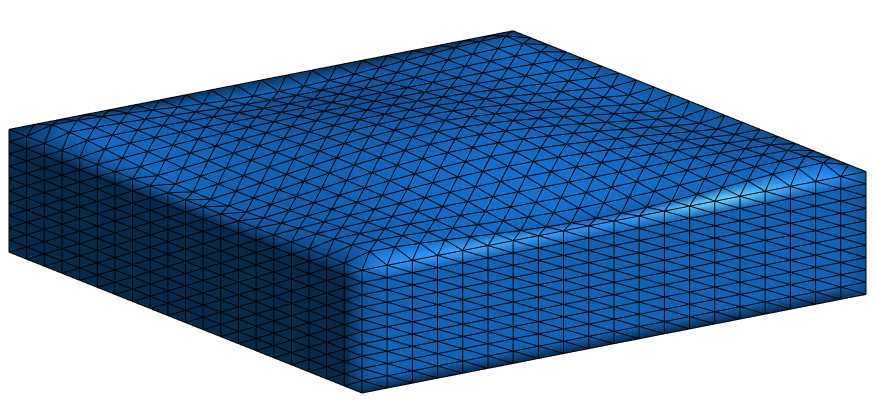
\includegraphics[width=.5\textwidth]{img/3D_cube_as_stl_cropped_1}
	\caption{Representation of the \texttt{.stl} file containing the prism used in the $3$D design optimization problem}
	\label{fig:3D_cube_stl_initial}
\end{figure}

This means that in order to modify the shape of the north face of the cube we can act on the height of its triangles control points (i.e. their vertices). Thus is useful to define the vector of the design variables as $\vec{l} = [l_1 \dots l_L]$ where $L \in \N$ is the number of triangle vertices which belongs to $\partial\Omega_\textup{flux}$ and the $i$-th variable $l_i \in \R$ control the height $z_i$ of the $i$-th vertex belonging to $\partial\Omega_\textup{flux}$. Defining the design variables in this way allows to define a finite-dimensional optimization problem which requires the definition of a cost function based on the variables $\vec{l}$ in order to be solved. We defined this cost function, which aims to approximate the one presented in equation~\eqref{eqn:continuous_3D_cost_function_results}, as:
\begin{equation}
	J = \frac{1}{\abs{A}} \sum_{j \in \mathcal{T}} \nabla \vec{u}(\vec{x}_j)^T \vec{a}_j
\end{equation}
where $\abs{A}$ is the area of $\partial\Omega_\textup{flux}$ computed as the sum of the areas of the triangles that belong to it, $\mathcal{T}$ is the set of the indices used to identify those triangles, $\nabla \vec{u}(\vec{x}_j)^T$ is the gradient vector of the field $u$ evaluated at $\vec{x}_j$, centroid of the $j$-th triangle, and $\vec{a}_j$ is the area vector of the $j$-th triangle which has direction given by its normal and modulus given by its surface.
Additionally the boundary value problem~\eqref{eqn:3D_BV_problem}, in general, must be discretized to be solved, doing so via RBF-HFD method yields the following constraint for the optimization:
\begin{equation}
	\label{eqn:3D_design_opt_constraint}
	\vec{C}_I\vec{u}_I + \vec{C}_B\vec{u}_B = \vec{f}
\end{equation}
where $\vec{u}_I$ and $\vec{u}_B$ are the vectors composed of the values of the field $u$ at the internal and boundary nodes, respectively, $\vec{C}_I$ and $ \vec{C}_B$ are the matrices representing the contribution of internal and boundary RBF-HFD nodes, respectively, and $\vec{f}$ is the vector composed of the values of $f$ at the internal nodes.
Therefore our overall design optimization problem reads as follow:
\begin{equation}
	\label{eqn:3D_design_opt_problem}
	\begin{aligned}
		\text{maximize} 		&  \quad J(\vec{u}, \vec{l})  									\\
		\text{by varying} 		&  \quad \vec{l}, \vec{u}_I, \vec{u}_B							\\
		\text{subject to}	 	&  \quad \vec{C}_I\vec{u}_I + \vec{C}_B\vec{u}_B = \vec{f}
	\end{aligned}
\end{equation}

\medskip
To solve problem~\eqref{eqn:3D_design_opt_problem} we have used a fixed number of $50$ optimization steps and $\vec{l}$ is updated using the following rule:
\begin{equation}
	\vec{l}_{k+1} = \vec{l}_k + \alpha \frac{\partial J}{\partial \vec{l}}
\end{equation}
where $\alpha$ is fixed heuristically, by trial and error, to $0.1$ and the vector $\partial J / \partial \vec{l}$ is computed as explained in subsection~\ref{subsec:adjoint_method_RBF-FD_3D}.
Constraint~\eqref{eqn:3D_design_opt_constraint}, on the other hand, is obtained employing the RBF-HFD method parametrized as follow:
\begin{itemize}
	\item the $N$ RBF-FD nodes scattered over the domain are generated according to the technique presented in~\cite{Zamolo:phd_thesis} which yields isotropic node distributions where equal node spacing is obtained along all directions. Unlike the $1$D case, thanks to this technique, the number of nodes scattered across the cube varies as the physical domain changes throughout the optimization;
	\item for the RBF basis we utilized the multiquadric function $\varphi(r) = \sqrt{1 + (\epsilon r)^2}$
	\item the degree of the polynomial augmentation is set to $P = 3$
	\item the number of nodes which constitute a single stencil is forced to $m = 50$.  % Obtained from rbfParameters in solutionInteractive.jl in AdjointMeshlessCube
\end{itemize}
The method also requires the solution of the sparse linear system reported in equation~\eqref{eqn:discretized_version_of_PDE_using_RBF-FD} for which we used the \verb|bicgstabl()| function present in the julia package called \verb|IterativeSolvers.jl|\footnote{Julia open source library which provides iterative algorithms for solving linear systems, eigensystems, and singular value problems. The project can be found at~\url{https://iterativesolvers.julialinearalgebra.org/stable/}.} setting \verb|GMRES|=2 and the left preconditioner \verb|Pl| set to \verb|ilu_LHS|; this function is an implementation of the iterative solver found in~\cite{Sleijpen:bicgstabl_paper} to which we refer for further details along with the \verb|IterativeSolvers.jl| package documentation.
As for the left preconditioner \verb|ilu_LHS|, it is the incomplete LU factorization of matrix $\vec{C}_I$ obtained via the \verb|ilu()| function of the \verb|IncompleteLU.jl|\footnote{Julia open source library which implements the Crout version of the incomplete LU factorization of a sparse matrix. The project can be found at~\url{https://github.com/haampie/IncompleteLU.jl}.} julia package with parameter $\boldsymbol{\tau}$ set to $6$. Its implementation is based on~\cite{NaLi:crout_ilu_paper}.
When \verb|ilu_LHS| is passed as parameter to \verb|bicgstabl()|, it is used to pre-multiply on the left both sides of equation~\eqref{eqn:discretized_version_of_PDE_using_RBF-FD} so as to accelerate the convergence to the solution of the iterative solver.

The results of the optimization, where the gradient at each step is computed employing the discreet adjoint method, are reported in figure~\ref{fig:opt_history_3D} where the values of the cost functions at each step are shown. Alongside, the values of the cost function obtained during the solution of the continuous design optimization problem solved through the continuous adjoint method are reported.

\begin{figure}
	\centering
	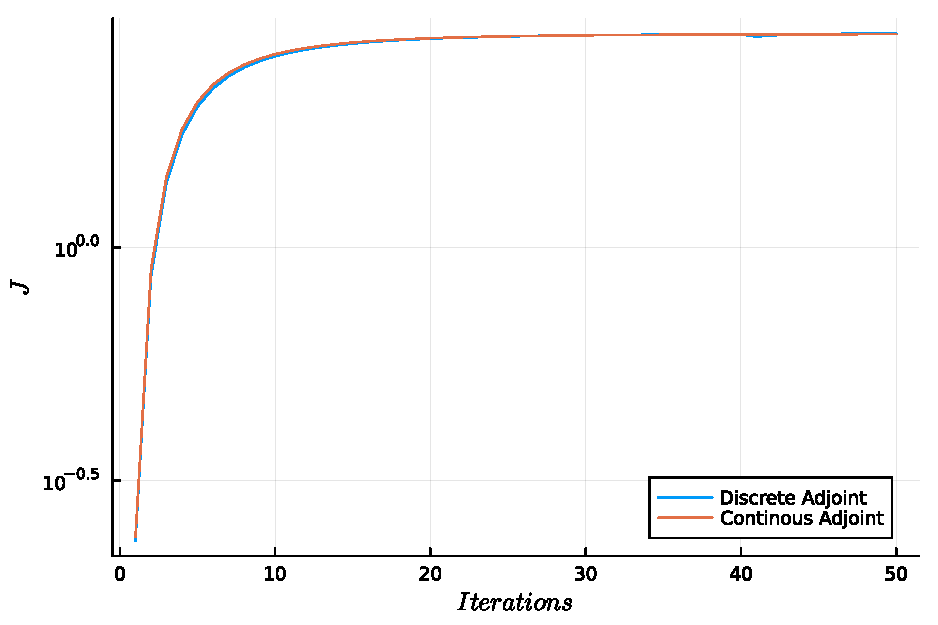
\includegraphics[width=.75\textwidth]{img/cost_vs_iter_3D_discrete_vs_continuous_adjoint}
%	\caption{Trajectories of the original (orange) and approximated (blue) cost functions throughout the optimization processes}
	\caption{Trajectories of the cost functions associated to the optimization problems obtained considering a prism defined in a continuous domain (orange, solved via continuous adjoint) and the same prism defined by means of a \texttt{.stl} file (blue, solved via discrete adjoint)}
	\label{fig:opt_history_3D}
\end{figure}
%TODO: Fixa la caption di questa figura. Dopo aver fixato metti che l'arancione è un tratto continuo, mentre il blu è tratteggiato

The deformations of surface $\partial\Omega_\textup{flux}$ at $4$ different times of the optimization are shown in figure~\ref{fig:3D_cube_shape_during_opt}.

\begin{figure}
	\centering
	\subfloat[][\emph{Surface after the first optimization step}]
	{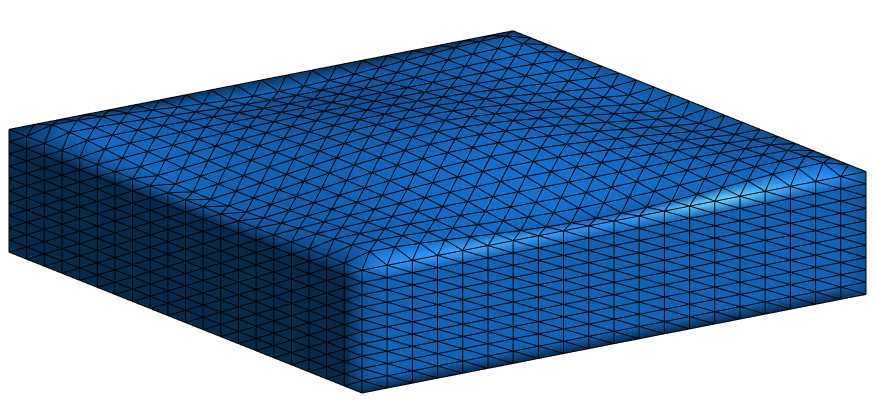
\includegraphics[width=.45\textwidth]{img/3D_cube_as_stl_cropped_1}} \quad
	\subfloat[][\emph{Surface after $N=5$ optimization steps}]
	{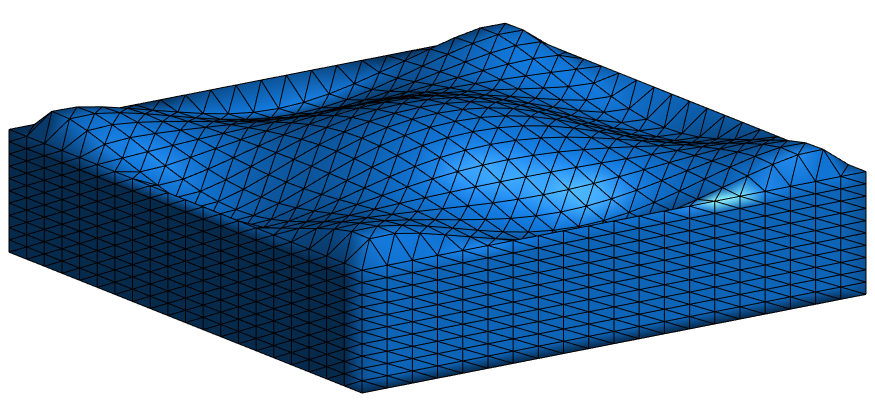
\includegraphics[width=.45\textwidth]{img/3D_cube_as_stl_cropped_5}} \\
	\subfloat[][\emph{Surface after $N=15$ optimization steps}]
	{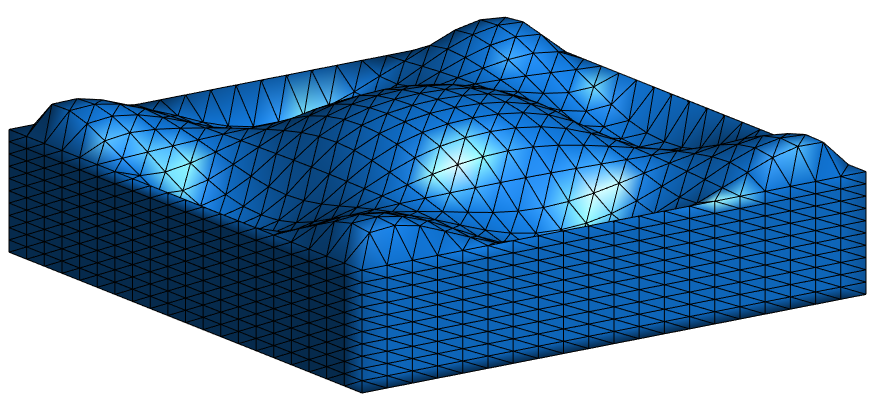
\includegraphics[width=.45\textwidth]{img/3D_cube_as_stl_cropped_15}} \quad
	\subfloat[][\emph{Surface after $N=50$ optimization steps}]
	{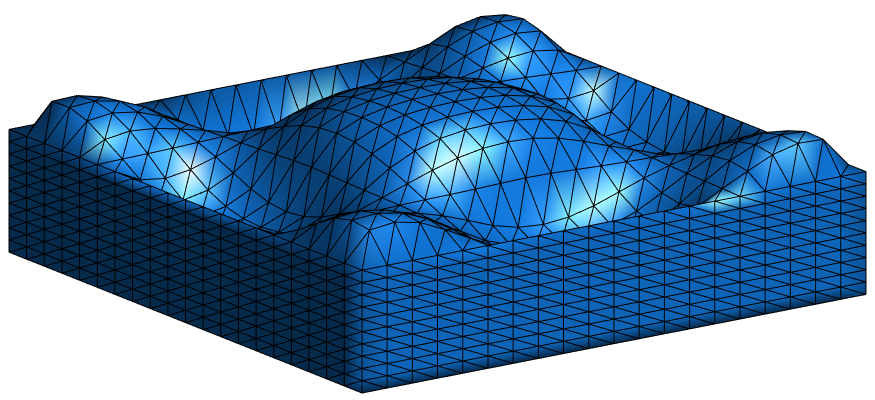
\includegraphics[width=.45\textwidth]{img/3D_cube_as_stl_cropped_50}}
	\caption{Deformation of the north face of the prism at different optimization times}
	\label{fig:3D_cube_shape_during_opt}
\end{figure}

%TODO: Chiedi a Davide:
%	0) Il problema di ottimizzazione infinito dimensionale è davvero un problema da risolvere?? E l'aggiunto continuo??
%	3) ilu di IncompleteLU.jl su quale paper si basa?? Cercando su internet ne vengono fuori 2. Uno con e uno senza
%	   pivotting. Nel dubbio ho citato quello con il pivotting che è più recente.